\documentclass[aps,prb,reprint,amsfonts,amsmath,amssymb,showpacs,groupedaddress,superscriptaddress]{revtex4-1}
\usepackage{bm}
\usepackage{color}
\usepackage{graphicx}
\usepackage[colorlinks,urlcolor=blue,linkcolor=blue,anchorcolor=blue,citecolor=blue,bookmarks]{hyperref}

\begin{document}

\title{Global phase diagram and possible quantum spin liquid in the triangular $J$-$K$-$\Gamma$ model}

\author{Shi Wang}
\affiliation{National Laboratory of Solid State Microstructures and School of Physics, Nanjing University, Nanjing 210093, China}

\author{\textcolor{cyan}{XXX}}
\affiliation{\textcolor{cyan}{XXX}}

\author{\textcolor{cyan}{XXX}}
\affiliation{\textcolor{cyan}{XXX}}

\author{Wei Wang}
\affiliation{School of Science, Nanjing University of Posts and Telecommunications (NUPT), Nanjing 210023, China}

\author{Shun-Li Yu}
\email{slyu@nju.edu.cn}
\affiliation{National Laboratory of Solid State Microstructures and School of Physics, Nanjing University, Nanjing 210093, China}
\affiliation{Collaborative Innovation Center of Advanced Microstructures, Nanjing University, Nanjing 210093, China}

\author{Jian-Xin Li}
\email{jxli@nju.edu.cn}
\affiliation{National Laboratory of Solid State Microstructures and School of Physics, Nanjing University, Nanjing 210093, China}
\affiliation{Collaborative Innovation Center of Advanced Microstructures, Nanjing University, Nanjing 210093, China}

\date{\today}

\begin{abstract}
The celebrated Kitaev honeycomb model provides an analytically tractable example with an exact quantum spin liquid ground state. While in real materials, other types of interactions besides the Kitaev coupling are present and these models can also be generalized to a triangular lattice. Here, we study the classical and quantum Heisenberg-Kitaev-$\Gamma$ model on a triangular lattice using the classical Monte Carlo and exact diagonalization. We find that the quantum phase diagram is quite similar to its classical counterpart in the large region, suggesting that the Kitaev physics would have emerged largely in the classical limit. Near the antiferromagetic (AF) Kitaev point, we show that the stripe order is selected out of the classic nematic order via the order-by-disorder mechanism. Around the AF $\Gamma$ point, we find a possible quantum spin liquid in a noticeable region with a continuum in spin excitations.
\end{abstract}

\maketitle

\section{\label{sec:Introduction}Introduction}
Geometric frustration, which arises when the lattice geometry gives rise to constraints that not every exchange bond can be simultaneously minimized in energy, plays an important role in various kinds of magnetic systems. The nearest-neighbor (NN) antiferromagetic (AFM) Heisenberg model on the triangular lattice is a typical example, once two of the spins on an elementary triangle are antiparallel to satisfy their antiferromagnetic interaction, the third one can no longer point in a direction opposite to both other spins. In particular, the special case where spins are $S=1/2$ has attracted numerous interests and was extensively studied after the seminal prediction by Anderson of a "quantum spin liquid" (QSL) where a strong quantum fluctuation prevents any long-range order down to the zero temperature~\cite{Anderson1973}, although it has been shown by later studies that the ground state (GS) have a classical magnetic order with each spin on a triangle pointing to 120$^\circ$ with respect to each other~\cite{PhysRevLett.99.127004,PhysRevLett.82.3899,PhysRevB.50.10048,PhysRevLett.60.2531}. When the second NN interactions are included which introduce further frustration, the system has a much richer phase diagram including the 120$^\circ$ N\'{e}el state, the stripe state and a QSL state~\cite{PhysRevB.91.014426,PhysRevB.92.041105,PhysRevB.92.140403,PhysRevB.96.165141,PhysRevB.93.144411,JPSJ.83.093707,PhysRevB.96.075116,PhysRevB.94.121111,PhysRevLett.123.207203}. All these studies have revealed that geometric frustated systems show quite different behavior from that of the non-frustated system.

On the other hand, exchange frustation in systems with strongly anisotropic magnetic interactions has been shown to be another promising approach to explore exotic quantum spin states. Like geometric frustation, the effect of exchange frustration is to prevent the formation of long range magnetic order and give raise to a residual ground-state entropy. The spin-$1/2$ Kitaev model~\cite{Kitaev2006} on honeycomb lattice, which has both gapped and gapless QSL states supporting fractionalized excitations, is a celebrated example of a model with exchange frustration. In this model, the spins subject to the Kitaev interactions consisting of nearest neighbor Ising-type interactions, with the quantization axis depending on the spatial orientation of an exchange bond. Because of its theoretical importance and potential application in quantum computing, great efforts have been made to search for a solid-state realization of the Kitaev model. G. Khaliullin \emph{et al.,}~\cite{Khaliullin2005,PhysRevLett.102.017205} proposed that this highly anisotropic Kitaev interaction can be realized in 4d/5d systems with a low spin state of $d^5$ configuration, such as iridates A$_2$IrO$_3$ (A = Na, Li). In these systems, the bond-directional interactions originate from the joint effects of strong spin-orbit coupling (SOC), electron interactions, $d^5$ configuration and 90$^\circ$ bond geometry formed by edge sharing octahedra. However, in real materials, other types of interaction besides the Kitaev coupling are present, and these interactions may induce other interesting ordered and disordered phases. The simplest extension of the pure Kitaev model is the Heisenberg-Kitaev (HK) model~\cite{PhysRevLett.105.027204}, in which the NN Heisenberg interaction is also taken into account. This model has been extensively studied by various numerical methods~\cite{PhysRevLett.110.097204,PhysRevB.83.245104,PhysRevB.84.100406,PhysRevB.90.195102,PhysRevLett.119.157203}, which reveal the presence of four magnetically ordered phases with collinear spin patterns of ferromagnetic (FM), AFM, stripy, and zigzag types, besides extended spin-liquid phases near the Kitaev limits. Considering the most idealized crystal structure, another interaction beyond the HK model also must be included, i.e. bond dependent symmetric off-diagonal exchange, which is called the $\Gamma$ interaction~\cite{PhysRevLett.112.077204,PhysRevB.93.214431,PhysRevB.96.115103}. Thus, the generic NN exchange Hamiltonian for the undistorted hexagonal compounds is the $J$-$K$-$\Gamma$ model, where the Heisenberg ($J$), Kitaev ($K$) and $\Gamma$ interactions are all included. Finite $\Gamma$ further enriches the phase diagram by adding non-collinear and incommensurate spiral phases~\cite{PhysRevLett.112.077204}. Moreover, in real materials, such as A$_2$IrO$_3$ and $\alpha$-RuCl$_{3}$, the dominant interactions are the $\Gamma$ and FM Kitaev terms which originate from both direct $d$-$d$ and anion mediated $d$-$p$ electron transfer, while the Heisenberg term has the smallest strength since it predominantly originates from the weak direct $d$-$d$ electron transfer~\cite{PhysRevLett.112.077204,PhysRevB.93.214431,PhysRevB.96.115103}.

In fact, magnetic ions located at the center of edge-shared octahedra can not only form the honeycomb lattice but also the triangular lattice (see Fig.~\ref{fig:ModelDefinition}(a)), so the Kitaev and $\Gamma$ terms can naturally be generalized to the triangular lattice~\cite{PhysRevB.89.014414,PhysRevB.93.104417}. The HK model ($\Gamma=0$) on the triangular lattice has been studied by means of Luttinger-Tisza minimization together with classical Monte Carlo simulation~\cite{PhysRevB.93.104417}, exact diagonalization~\cite{KaiLi2015}, and density matrix renormalization group~\cite{JPSJ.85.114710,PhysRevX.9.021017}. All these methods give consistent results about four magnetically ordered phases: two collinear patterns of FM and stripy types, and two noncollinear patterns of 120$^\circ$ N\'{e}el and noncoplanar spiral types. Note that the distortions of the 120$^\circ$ N\'{e}el order, when the model deviates from the AFM Heisenberg limit ($K=0$, $J>0$), were also called the $Z_{2}$ vortex crystal~\cite{PhysRevB.93.104417,JPSJ.85.114710}. However, the nature of the phase around the antiferromagnetic Kitaev point is still under debate. The Luttinger-Tisza minimization method suggested it to be a $Z_{2}$ vortex crystal~\cite{PhysRevB.93.104417}, the Schwinger-fermion mean-field theory proposed it to be a QSL~\cite{KaiLi2015}, while the density matrix renormalization group calculations suggested it to be a nematic phase~\cite{JPSJ.85.114710} or a stripe phase~\cite{PhysRevX.9.021017}. When the symmetric off-diagonal exchange interaction $\Gamma$ is included, a classical analysis reveals that the stripe and ferromagnetic phases dominate the $J$-$K$-$\Gamma$ phase diagram, in addition to small regions of 120$^\circ$, $Z_{2}$ vortex crystal and nematic phases~\cite{PhysRevB.92.165108}. However, the studies on the effects of quantum fluctuations on the global $J$-$K$-$\Gamma$ phase diagram are scarce. In particular, since no exact solution has been reported so far for the pure spin-$1/2$ Kitaev and $\Gamma$ models on the triangular lattice, it also remains conceptually interesting to investigate whether QSL states could exist as possible GSs due to quantum fluctuations introduced by these exchange-frustrated interactions.

\begin{figure}
    \centering
    \begin{minipage}{0.6\columnwidth}
        \includegraphics[width=\linewidth]{fig/EdgeSharingOctahedrons.pdf}
    \end{minipage}\hspace{0pt}
    \begin{minipage}{0.3\columnwidth}
        \includegraphics[width=\linewidth]{fig/SingleOctahedron.pdf}\vspace{0pt}
        \includegraphics[width=\linewidth]{fig/ModelDefinition.pdf}
    \end{minipage}
    \caption{\label{fig:ModelDefinition}(Color online) (a) Top view of the triangular lattice of the edge-sharing octahedron. (b) The orientation of the cubic $x$, $y$, $z$ axes with respect to the octahedron. The spin operators $S^x$, $S^y$ and $S^z$ are defined with respect to this reference frame. (c) Three types of the NN bonds on the triangular lattice, namely $\gamma=x, y, z$ colored red, green and blue, respectively. The different colors of the lattice sites label the four sublattices realizing the four-sublattice-transformation, see the main text for detailed information.}
\end{figure}

On the experimental side, studies of several classes of rare-earth compounds have recently shown that the quantum spin model on the triangular lattice can be formed by $4f$ moments. In particular, due to their possible Kramers doublets and spin-orbital coupling, the $4f$ electrons can be treated as $S_{eff}=1/2$ at low temperatures, and the spin-orbit entanglement can induce direction-dependent exchanges, such as the $K$ and $\Gamma$ terms. A typical example is YbMgGaO$_{4}$~\cite{srep16419,PhysRevLett.115.167203,PhysRevLett.117.097201,nphys3971,Nature20614,PhysRevLett.117.267202,PhysRevLett.120.087201,PhysRevLett.122.137201,LiAdroja-398}, in which the Yb$^{3+}$ ions form a triangular layer and are surrounded by O$^{2-}$ which construct edge sharing octahedra~\cite{srep16419,PhysRevLett.115.167203}. At low temperatures, QSL states have been proposed due to its lack of long-range magnetic order and the observation of a continuum of magnetic excitations~\cite{srep16419,PhysRevLett.115.167203,PhysRevLett.117.097201,nphys3971,Nature20614}, but the exchange disorder induced by the intermixture of Mg$^{2+}$ and Ga$^{3+}$ may lead to a spin glass state~\cite{PhysRevLett.120.087201} or a random valence bond state~\cite{PhysRevLett.122.137201,LiAdroja-398}. More recently, an alternative family of compounds AReCh$_2$ (A=alkali, Re=rare-earth, Ch=O, S, Se) with perfect triangular lattices of rare-earth ions have been synthesized and explored. The magnetic susceptibilty and heat capacity data suggest no long-range magnetic order or spin freezing down to the lowest measurement temperature, which implies their candidacy for QSL state~\cite{acsmaterialslett.9b00464,PhysRevMaterials.3.114413,arXiv1911.08036,Liu_2018,PhysRevB.99.180401,PhysRevB.100.224417,PhysRevB.100.144432}. These triangluar magnets of rare-earth ions provide suitable platforms to study the interplay of geometric frustation and exchange frustration induced by spin-orbit coupling.

{
    \color{red}The rest of the paper is organized as follows: In Sec.~\ref{sec:Model} we introduce the $J$-$K$-$\Gamma$ model as well as the four-sublattice-transformation that can be applied to the HK model. The exact diagonalization and classical Monte Carlo methods are introduced in Sec.~\ref{sec:Methods}. Section~\ref{sec:Results} disscuss the main results of this paper.
}

\section{\label{sec:Model}Model}

The $J$-$K$-$\Gamma$ model Hamiltonian on the triangular lattice is given by
\begin{equation}
    H = \sum_{\langle i,j \rangle \in \alpha \beta (\gamma)} \lbrack J \bm{S}_i \cdot \bm{S}_j + K S_i^{\gamma} S_j^{\gamma} + \Gamma (S_i^{\alpha} S_j^{\beta} + S_i^{\beta} S_j^{\alpha}) \rbrack,
    \label{eq:Hamiltonian}
\end{equation}
where $\langle i,j \rangle$ denotes the NN bonds, $\gamma$ takes value $x$, $y$, or $z$ depending on the direction of the NN bond as shown in Fig.~\ref{fig:ModelDefinition}(c), and $\alpha$, $\beta$ are the remaining directions. $J$ and $K$ are the magnitude of the Heisenberg and Kitaev interactions, and $\Gamma$ the symmetric off-diagonal exchanges.

In the followings, for convenience, we fix the energy scale with $\sqrt{J^2 + K^2 + \Gamma^2}=1$ and parametrize the exchange interactions using spherical angles $\alpha$ and $\beta$
\begin{equation}
    J = \sin\alpha \sin\beta, \quad
    K = \sin\alpha \cos\beta, \quad
    \Gamma = \cos\alpha
    \label{eq:Parameters}
\end{equation}
where $\alpha \in [0, \pi]$ and $\beta \in [0, 2\pi]$ to cover the global parameter space.

In the HK limit ($\Gamma=0$), the model~\eqref{eq:Hamiltonian} admits an exact duality transformation, i.e., the so-called four-sublattice-transformation (FST)~\cite{PhysRevB.89.014414}. The FST is a spin rotation transformation which divides the triangluar lattice into four sublattices (see Fig.~\ref{fig:ModelDefinition}(c)) and performs the following rotations of the spins on the four sublattices to map the spin $\bm{S}_{i}$ to $\bm{S}_{i}^{\prime}$,
\begin{align*}
    & \bm{S}_{0}^{\prime} = \bm{S}_{0}& \quad \text{for sublattice 0}, \\
    & \bm{S}_{1}^{\prime} = (S_1^x, -S_1^y, -S_1^z)& \quad \text{for sublattice 1}, \\
    & \bm{S}_{2}^{\prime} = (-S_2^x, S_2^y, -S_2^z)& \quad \text{for sublattice 2}, \\
    & \bm{S}_{3}^{\prime} = (-S_3^x, -S_3^y, S_3^z)& \quad \text{for sublattice 3}.
\end{align*}
This corresponds to a $\pi$ rotation around $x$, $y$, and $z$ axis for the sublattices $1$, $2$, and $3$, respectively. The resulting Hamiltonian $H^{\prime}(\bm{S}^{\prime})$ has the same form as the original Hamiltonian albeit with different model parameters $J^{\prime} = -J$ and $K^{\prime} = 2J + K$. For the spherical angles defined in Eq.~\eqref{eq:Parameters}, the mapping takes the form
\begin{align}
    \tan\beta^{\prime} = -\sin\beta / (2\sin\beta + \cos\beta).
    \label{eq:FST}
\end{align}
This special property of the model can help us to identify some exotic magnetically ordered phases from the well established simple counterparts.

\section{\label{sec:Methods}Methods}

\subsection{\label{subsec:MethodED}Exact Diagonalization}

To obtain the quantum phase diagram of the model~\eqref{eq:Hamiltonian}, we perform exact-diagonalization calculations of the GS of the Hamiltonian~\eqref{eq:Hamiltonian} on a $4 \times 6$ cluster with the periodic boundary condition. To detect quantum phase transitions, the second derivatives of the GS energy, $-\partial^2E_0/\partial\alpha^2$ and $-\partial^2E_0/\partial\beta^2$ were computed and its singularities are used to identify possible phase transtions.

To identify the ground-state properties, we first examine the static structure factor (SSF),
\begin{align}
    \mathcal{S}(\bm{Q}) = \frac{1}{N} \sum_{ij} \langle \Omega | \bm{S}_i \cdot \bm{S}_j | \Omega \rangle e^{i \bm{Q} \cdot (\bm{R}_i - \bm{R}_j)},
    \label{eq:SSF}
\end{align}
from which we can find the wave vectors of the ordered phases and distinguish possible QSL states. Here, $|\Omega\rangle$ is the GS, $N$ is the total number of lattice sites, and $\bm{R}_i$ the position of site $i$.

To further determine the magnetic configurations of the magnetically ordered phases, we employ a method by studying the projections of the exact GSs of the finite cluster to the classical states~\cite{PhysRevB.94.064435}. The basic idea of this method is to measure the probabilities of the exact cluster GS on cluster spin-coherent states with varying moment directions. The cluster spin-coherent state is a direct product of spin-1/2 coherent states on each site $i$, i.e.,
\begin{align}
    |\Psi \rangle = \bigotimes_{i=1}^N | \theta_i, \phi_i \rangle,
    \label{eq:ClusterCoherentState}
\end{align}
where the spin-1/2 coherent state
\begin{align}
    |\theta, \phi\rangle = \mathcal{R}_z(\phi) \mathcal{R}_y(\theta) | \uparrow \rangle = e^{-i \phi S^z} e^{-i \theta S^y} | \uparrow \rangle
    \label{eq:Spin-1/2CoherentState}
\end{align}
is fully polaried state along the $(\theta, \phi)$ direction. Here the cubic axes are used (see Fig.~\ref{fig:ModelDefinition}(b)), $\theta$ and $\phi$ are the conventional spherical angles. By calculating the overlap between the exact cluster GS and cluster spin-conherent states, $P = | \langle \Psi | GS \rangle|^2$, and maximizing its value with respect to $\theta$'s and $\phi$'s, we can then identify the classical spin pattern that best fits the exact quantum GS.

Since one of the key characteristics of QSL is the fractional excitation, which can lead to a continuous spectrum, so we study the dynamic structure factor (DSF) $A(\bm{k}, \omega)$ to search for the possible QSLs. $A(\bm{k}, \omega)$ is given by
\begin{align}
    & A(\bm{k}, \omega) = -\frac{1}{\pi} \text{Im} \mathcal{S}(\bm{k}, \omega), \label{eq:Akomega} \\
    & \mathcal{S}(\bm{k}, \omega) = \frac{1}{N} \sum_{ij} \mathcal{S}_{ij}(\omega) e^{i \bm{k} \cdot (\bm{R}_i - \bm{R}_j)}, \\
    & \mathcal{S}_{ij}(\omega) = \langle \Omega | S_i^{+} \frac{1}{\omega + i0^{+} - H + E_0} S_j^{-} | \Omega \rangle, \label{eq:GreenFunction}
\end{align}
where $E_0$ is the ground state energy.

\subsection{\label{subsec:MethodMC}Classical Monte Carlo}

In order to better understand the quantum phases identified by the exact diagonalization method, we also perform classical Monte Carlo simulations. We begin with paralleling-tempering Monte Carlo~\cite{Hukushima96} on 40 replicas with temperature $T/J$ ranging from $0.001$ to $1.0$. For each replica, we sample it with a combination of heat-bath~\cite{Miyatake84} and over-relaxation method~\cite{Berg} mainly on a $24\times 24$ triangle lattice with periodic boundary conditions. A whole MC step consists of a single heat-bath sweep and subsequent 10 over-relaxation sweeps over the entire lattice. We perform $10^6$ MC steps per replica, then, we copy out the spin configuration from the lowest-T replica, and sample it with a combination of zero-temperature heat-bath and over-relaxation method to get the GS. The zero-temperature heat-bath sampling is simply aligning the spins according to their local fields:
\begin{align}
    \bm{S}_i = \frac{\bm{h}_i^{loc}}{|\bm{h}_i^{loc}|} S,
\end{align}
with
\begin{align}
    \bm{h}_i^{loc} = \sum_{\langle j \rangle} J \bm{S}_j + K {S}^{\gamma}_j \hat{e}^{\gamma} + \Gamma (S^\alpha_j \hat{e}^{\beta} + S^\beta_j \hat{e}^\alpha),
\end{align}
For some competing states, we start from several different initial configurations in order to obtain the correct classical GS.

From the magnetic configuration of GS, we compute the spin structure factor given by
\begin{align}
    \mathcal{S}_{\bm{k}} = \frac{1}{N} \sum_{ij} \left \langle \bm{S}_i \cdot \bm{S}_j \right \rangle e^{i \bm{k} \cdot (\bm{r}_i-\bm{r}_j)},
\end{align}
which is a key characterizes to identify magnetic phases.

\section{\label{sec:Results}Results}

\subsection{\label{subsec:GlobalPhaseDiagram}Global Phase Diagram}

\begin{figure*}
    \centering
    \includegraphics[width=\textwidth]{fig/QuantumGlobalPhaseDiagram.pdf}
    \caption{\label{fig:QuantumPhaseDiagram}(Color online) Global phase diagram of the triangular lattice $J$-$K$-$\Gamma$ model. The angle $\alpha$ and $\beta$ denote the radial and azimuthal angles, respectively. There are in total nine phases including three different FM phases denoted as FM-A, FM-B and FM-C, three different stripe phases designated as Stripe-A, Stripe-B and Stripe-C, 120$^\circ$ N\'{e}el, Dual N\'{e}el and a possible quantum spin liquid phase. The three FM phases different from each other in the direction of the ordered moment, and also the three stripe phases are distinguished by their moment directions, see main text for details.}
\end{figure*}

The quantum phase diagrams obtained by the exact-diagonalization method for $\Gamma \geq 0$ and $\Gamma \leq 0$ are presented in Fig.~\ref{fig:QuantumPhaseDiagram}. The phase boundaries are obtained from the location of singularities in $-\partial^2E_0/\partial\alpha^2$ and $-\partial^2E_0/\partial\beta^2$.

In the HK limit ($\Gamma=0$), as with the previous study~\cite{KaiLi2015}, we find five quantum phases. For pure Heisenberg models ($K=\Gamma=0$), the GSs are well known, i.e., a FM state for $J<0$ and a 120$^\circ$ N\'{e}el state for $J>0$. As mentioned in Sec.~\ref{sec:Model}, the form of the HK model ($\Gamma=0$) is invariant under the FST~\cite{PhysRevB.89.014414} but with different exchange interactions. Thus, by virtue of the FST, two more magnetic ordered phases can be identified. When $\beta=\pi - \arctan\frac{1}{2}$ in Eq.~\eqref{eq:FST}, the FST maps the Hamiltonian~\eqref{eq:Hamiltonian} to FM Heisenberg model of the rotated spin operators $\bm{S}^{\prime}$, whose GS is a FM state. Thus, transformating back to the original spin basis, a collinear stripe order can be obtained. Similarly, a noncollinear spiral order (dual N\'{e}el) is obtained from the 120$^\circ$ N\'{e}el order for $\beta=-\arctan\frac{1}{2}$. However, for the phase near the AFM Kitaev point ($J=\Gamma=0$, $K>0$), it is mapped to itself under FST, so we can not identify its magnetic properties with the FST.

When the $\Gamma$ term is included, we find that the stripe phase, the FM phase and the phase near the AFM Kitaev point in the HK model are actually phase boundaries in the global phase diagram of the $J$-$K$-$\Gamma$ model. Moreover, except the 120$^\circ$ N\'{e}el state and the dual N\'{e}el state, which already exist in the HK limit, there are six other new phases.

To reveal the natures of these new phases, we perform the classical MC calculations as described in Sec.~\ref{subsec:MethodMC}. For convenience of comparison between the quantum and classical results, we also present the classical phase diagram obtained from the MC simulations in Fig.~\ref{fig:ClassicalPhaseDiagram}, which is consistent with the phase diagram reported in Ref.~\onlinecite{PhysRevB.92.165108}. According to the classical MC results, we can identify that the three new phases with large areas mainly located in the $J>0$ region have stripe orders (i.e., the stripe-B and stripe-C phases), while the two new phases mainly located in the $J<0$ region are FM (i.e., the FM-A and FM-C phases). In addition, we find that the area of the 120$^\circ$ N\'{e}el state in the quantum phase diagram is greatly reduced, and more importantly the extra phase near $\Gamma=1$ that does not exist in the classical phase diagram.
\begin{figure}
    \centering
    \includegraphics[width=\columnwidth]{fig/ClassicalGlobalPhaseDiagram.pdf}
    \caption{\label{fig:ClassicalPhaseDiagram}(Color online) Classical global phase diagram of the $J$-$K$-$\Gamma$ model obtained from classical Monte Carlo simulation.}
\end{figure}

\begin{figure}
    \centering
    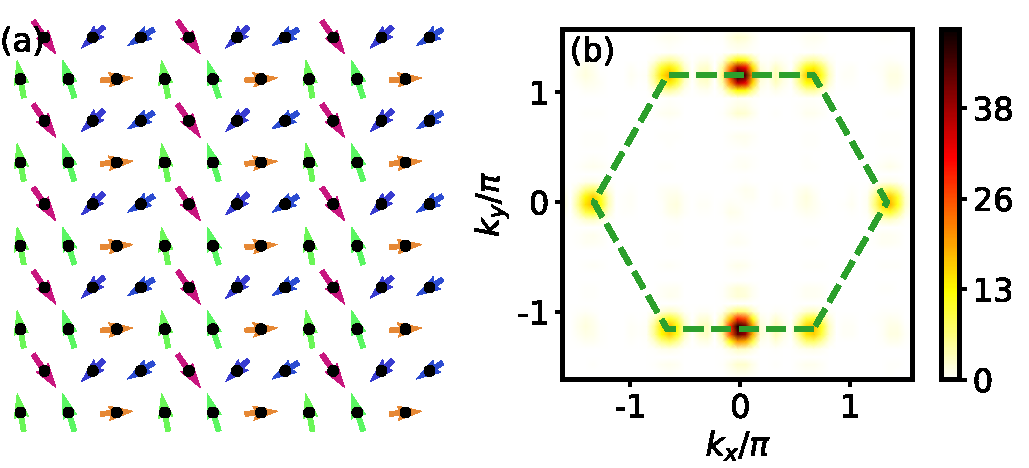
\includegraphics[width=\columnwidth]{fig/SixSitesOrder.pdf}
    \caption{\label{fig:SixSitesOrder}(Color online) Spin configuration and spin structure factor for \emph{six-chains stripe order}. The green dashed line in (b) marks the first Brillouin Zone.}
\end{figure}

The properties of each quantum phases, especially the spin configuration of the ordered phases, can also be inferred from the SSF in~\eqref{eq:SSF},  so we illustrate the results for some typical parameters in Fig.~\ref{fig:StructureFactors}. The results in Fig.~\ref{fig:StructureFactors}(d) and (e) show the SSFs in the stripe-B and stripe-C phases, respectively. It is clear that the SSFs are peaked at the $\tilde{M}$ points of the first Brillouin zone (BZ), which is a typical characteristic of stripe ordered states. For the case of pure AFM Kitev limit ($J=\Gamma=0$, $K=1$), the SSF in Fig.~\ref{fig:StructureFactors}(a) shows the same structure as those in Fig.~\ref{fig:StructureFactors}(d) and (e), so the GSs around the AFM Kitev point also belongs to a stripe phase, which we label the stripe-D phase. In Fig.~\ref{fig:StructureFactors}(b) and (c), we show the results of two other special points with $\Gamma=\pm1$ and $J=K=0$, i.e., the pure $\Gamma$ models. We find that the GSs of both models have ferromagnetic order, as the SSFs are peaked at $\tilde{\Gamma}$ point of the first BZ. The ferromagnetic phases contains these two specail points are denoted with FM-A and FM-C in Fig.~\ref{fig:QuantumPhaseDiagram}(a). The SSF for the quantum phase that does not exist in the classical phase diagram in a small region around the point with $J=K=0$ and $\Gamma=1$ is illustrated in Fig.~\ref{fig:StructureFactors}(f), which exhibits high intensities at both $\tilde{\Gamma}$ and $\tilde{M}$. {\color{red}It seems impossible for a classical magnetically ordering state to satisfy these two wave vectors simultaneously, so we infer that this quantum phase is a QSL.}
\begin{figure}
    \centering
    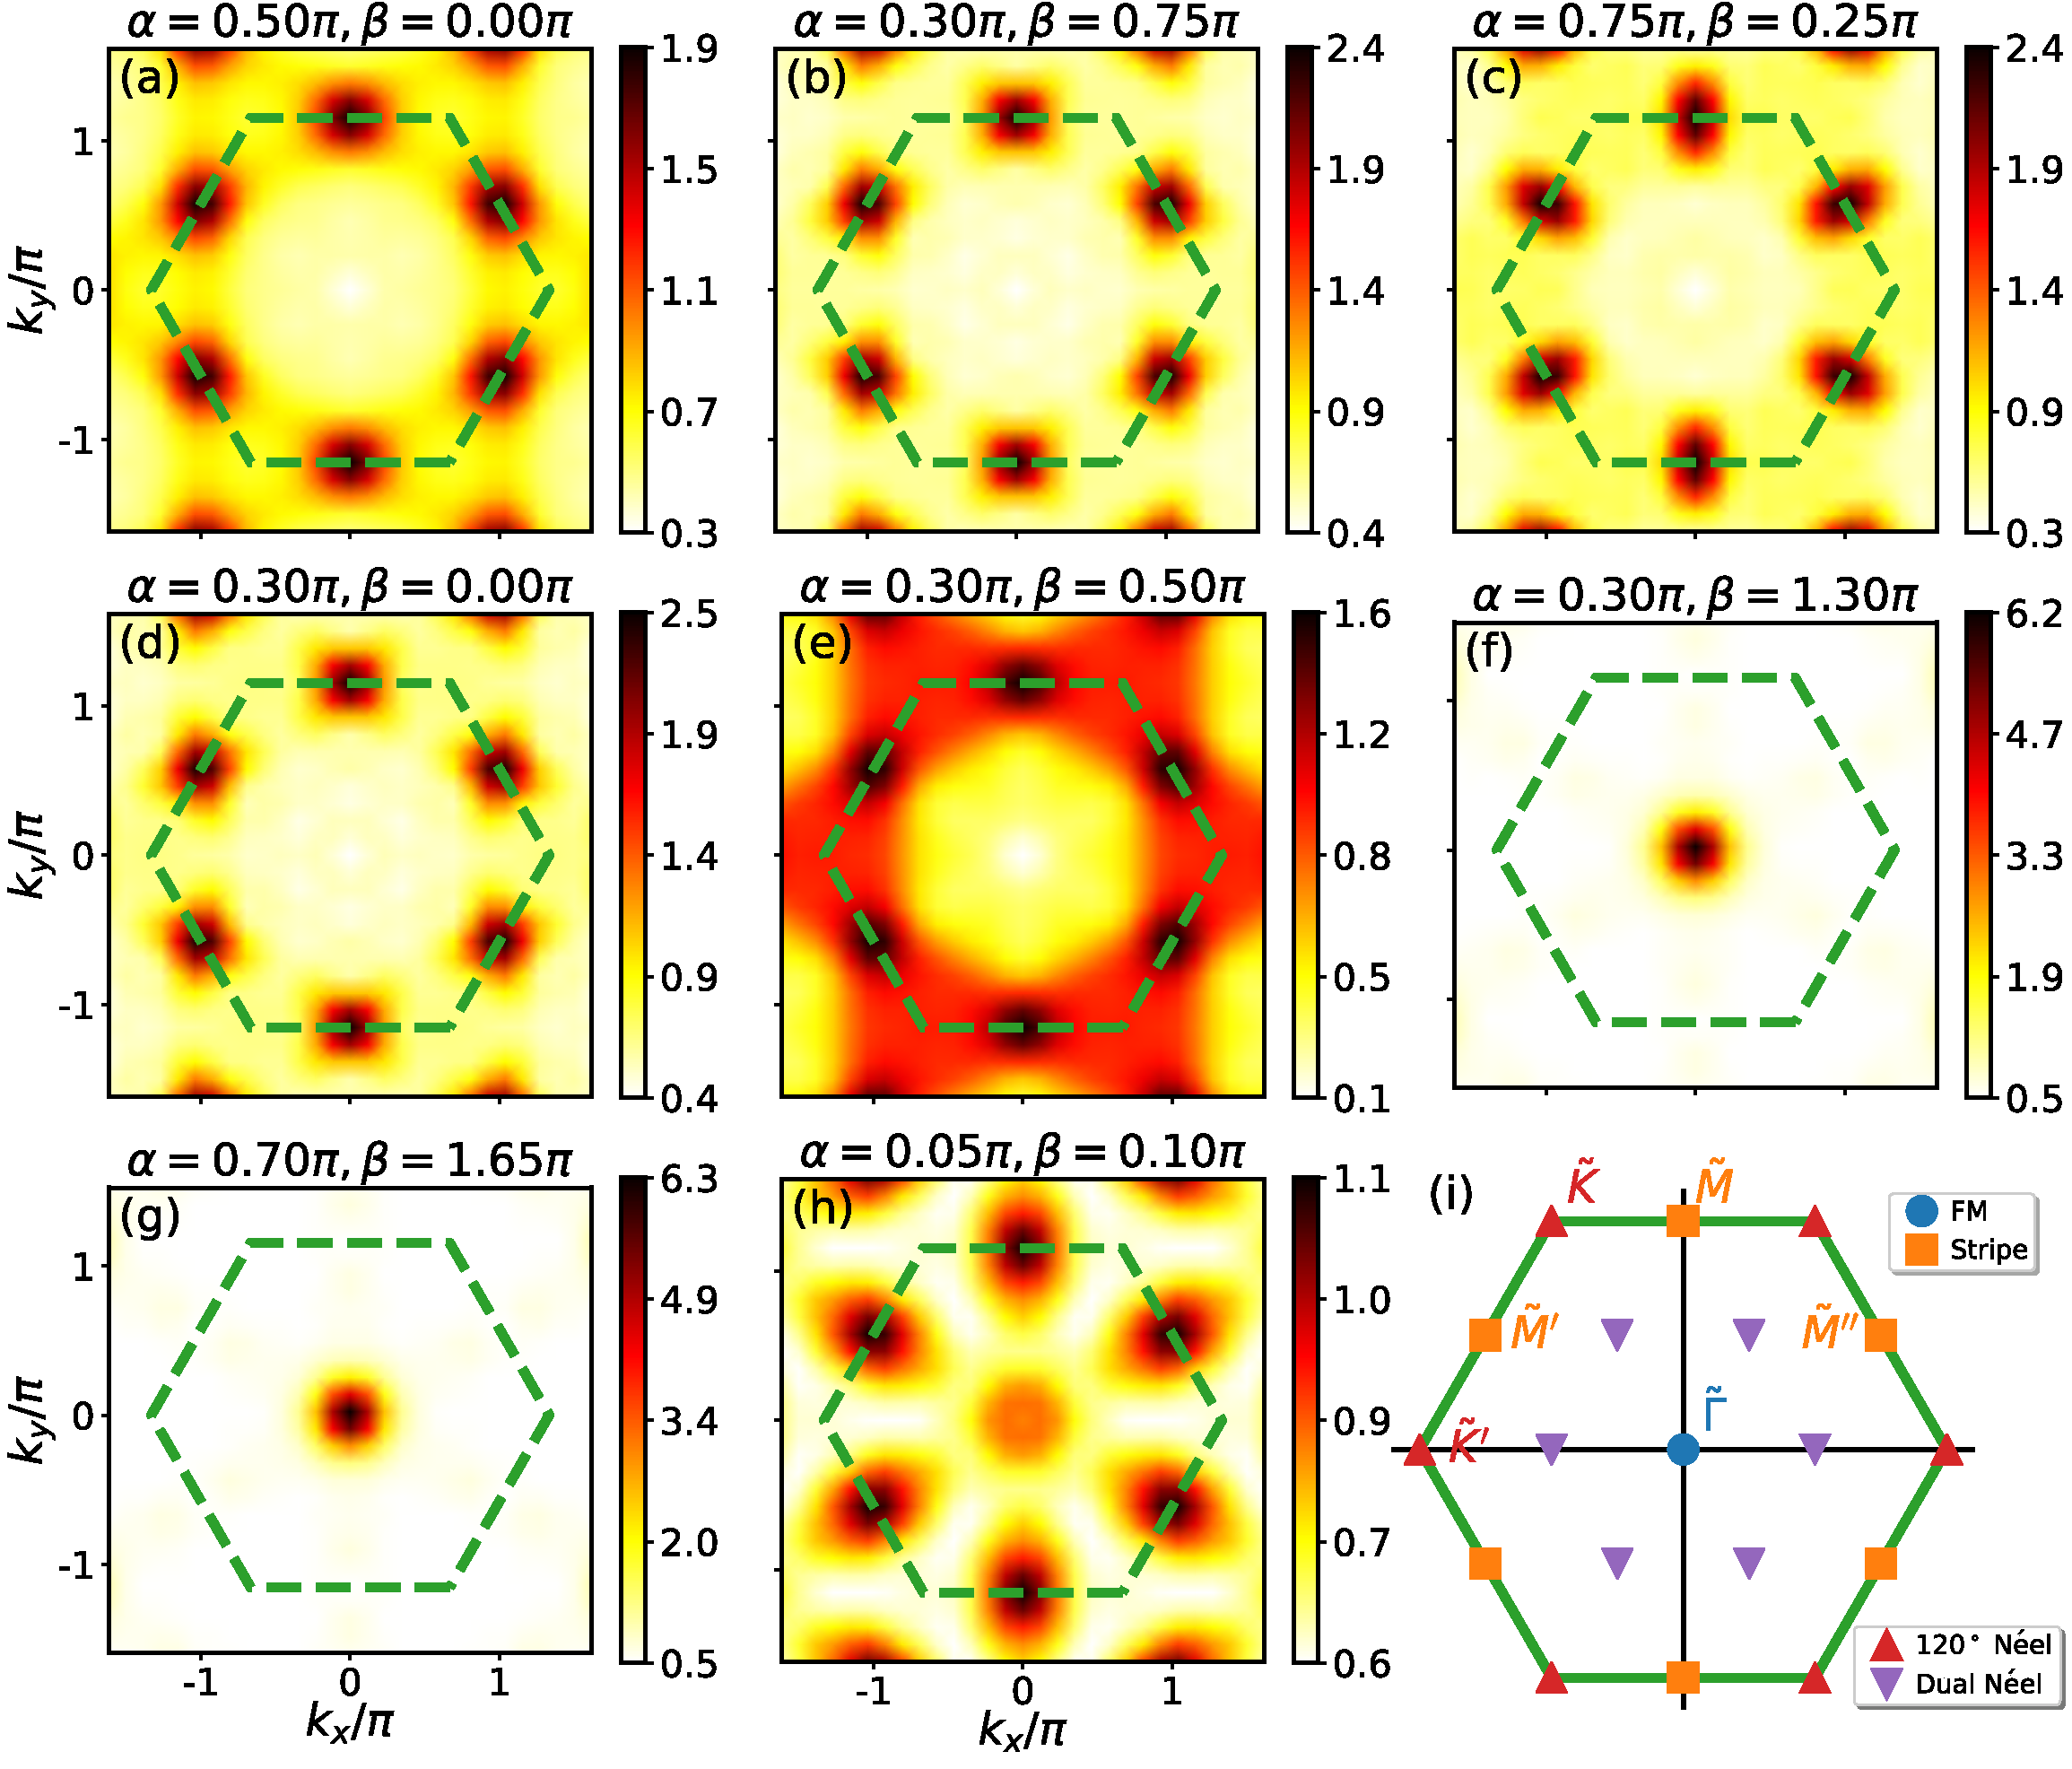
\includegraphics[width=\columnwidth]{fig/StructureFactors.pdf}
    \caption{\label{fig:StructureFactors}(Color online) SSF for different model paramters. The green dashed lines marks the first BZ corresponding to the triangular lattice.}
\end{figure}

According the above analysis, we find that, unlike the case for the honeycomb lattice, the Kitaev interactions on the triangular lattice do not give rise to QSL states, so the quantum phase diagram is similar to its classic counterpart. Here, the large coordination number plays a key role to stabilize the classical magnetic order, although the geometric and exchange frustrations coexist in the triangular lattice $J$-$K$-$\Gamma$ model. Although we have basically determine the nature of each phase, there are still two problems should be explained: first, why there are phase transitions between the phases with the same type of classical order, suas the phase transitions between FM phases and stripe phases; second, what other important characteristics of the QSL phase in the phase diagram can be used to help us understand its properties more deeply. In the followings, we will address these problems.

\subsection{\label{subsec:FMPhases}FM Phases}

To have a better understanding of the phase transitions between these FM phases, we first study the classical $J$-$K$-$\Gamma$ model where the spin operators are viewed as unit-vectors in three dimension. For classical FM states, all spins are aligned in parallel and the energy of the $J-K-\Gamma$ model per lattice site is given by
\begin{equation}
    E_{FM}^{c} = (3J + K) + 2 \Gamma (v^x v^y + v^y v^z + v^z v^x) \label{eq:EcFM}
\end{equation}
where $v^x$, $v^y$, $v^z$ are the corresponding components of the classical moment vector. On this level, the moment direction of the classical FM state is determined solely by $\Gamma$ and the problem becomes finding the global minimum and maximum of the multi-variable function $f(v^x, v^y, v^z) = v^x v^y + v^y v^z + v^z v^x$ with the constraint $|\bm{v}| = 1$. $f(v^x, v^y, v^z)$ takes maximum value $f_{max}=1$ at $v^x=v^y=v^z=\pm 1/\sqrt{3}$ and minimum value $f_{min}=-0.5$ when the conditions $v^x + v^y + v^z = 0$ and $|\bm{v}| = 1$ are fulfilled. The condition $v^x + v^y + v^z = 0$ specifies a plane that passes the coordinate origin and is perpendicular to the $[111]$ direction. Considering the reference frame shown in Fig.~\ref{fig:ModelDefinition}(b) this is actually the plane of the triangular lattice. That is to say, for $\Gamma > 0$ the ordered moment of the classcial FM state prefers to lie in the lattice plane and when $\Gamma$ is negative, the ordered moment would perpendicular to the lattice plane.

Our classical Monte Carlo simulation found FM ordered states with the right moment direction for majority of the area marked as FM phase (see Fig.~\ref{fig:ClassicalPhaseDiagram}) except for the pure $\Gamma$ term. For pure positive $\Gamma$ interaction, apart from the FM order lie in the lattice plane, we also found disordered states which have the same energy as the FM state but no states with lower energy were found. When $\Gamma=-1$, in addition to the FM order perpendicular to the lattice plane, other long-range ordered states which are energetically degenerate with the FM state appear (see Appendix~\ref{apx:DegeneratedStates} for details). Based on these observation, it is reasonable to say that the GS of the classical $\Gamma$ model is highly degenerate though the degeneracy may be lifted by introducing other interactions. For example, a ferromagnetic ($J<0$) Heisenberg interaction would break the degeneracy and select the FM ordered state as the GS. On the other hand, when positive Heisenberg interaction is included, which introduces further frustation to the system, the FM order is unlikely to be the GS.

In light of the classical analysis, we conjecture the main differences between these FM phases lies in the ordered moment direction. To further confirm our hypothesis, we employ the method developed by Ji\v{r}\'{i} Chaloupka \emph{et  al} \cite{PhysRevB.94.064435} to extract the moment direction of these FM phases from our ED cluster ground state. Since the cluster spin-coherent state is captured only by a single pair of $(\theta, \phi)$ for collinear states (such as FM and stripe), it is easy to determine the direction of the ordered moment by inspecting the probability map $P(\theta, \phi) = | \langle \Psi (\theta, \phi) | GS \rangle |^2$. The resulting probability maps for representive model parameters of FM-A and FM-C phases are shown in Fig.~\ref{fig:Proabilities}(a) and (b). It is worth to note that the large overlap between the exact cluster GS and FM ordered cluster spin-coherent state again provides solid evidence that the corresponding areas are FM phases. For pure Heisenberg model, the FM state is spin rotational invariant and the ordered moment can point any direction. The easy axis Kitaev interaction breaks the accidental spin rotational symmetry, pinning the orderings to the axis direction (i.e., $x$, $y$, $z$ direction). In other words, the ordered moment of the FM-B phase is in the direction of the $x,y,z$-axis. However, when the off-diagonal $\Gamma$ term is introduced, which would compete with Kitaev interaction, the moment orientation will deviate from the axis direction. For the FM-A phase, the probability map reveals the moment being constrained to the lattice plane (marked by the green dashed line in Fig.~\ref{fig:Proabilities}(a)) with all directions degenerate. The probability map for the FM-C phase is clearly peaked at the direction perpendicular to the lattice plane (marked by the green solid circle in \ref{fig:Proabilities}(b)). The ground states of the quantum model in these areas are similar to their classical analogue except for the pure $\Gamma$ model. For $\Gamma=1$, the GS of the classical model is highly degenerate including FM ordered states and states with no long range order. However, for the quantum model, quantum flucations select the FM ordered states lie in the lattice plane as GS out of an otherwise infinitely degenerate manifold of classical states. Similarly, the degeneracy for the classical model at $\Gamma=-1$ is lifted by quantum flucations and the FM state perpendicular to the lattice plane is selected as the GS. This selection of states among degenerate classical ground states is the so called \emph{order-from-disorder} mechanism previously emphasized by Villain and Henley in the context of the square lattice XY model \cite{PhysRevLett.62.2056} and by Oguchi \emph{et al.,} in the case of fcc antiferromagnet \cite{JPSJ.54.4494}.

In the HK limit, the GS of the model near the $J=-1$ point is FM state and the ordered moment is fixed to the $x,y,z$-axis direction by the Kitaev interaction. When an infinitesimal $\Gamma$ interaction is introduced, positive couplings drive the ordered moment to the lattice plane and negative couplings pinning the ordered moment to be perpendicular to the lattice plane.

\begin{figure}
    \centering
    \includegraphics[width=\columnwidth]{fig/Probabilities.pdf}
    \caption{\label{fig:Proabilities}(Color online) Map of the probabilities of the cluster spin-coherent state given by Eq.~\eqref{eq:ClusterCoherentState} in varies exact cluster GS. The radial and polar coordinate gives the angles $\theta$ and $\phi$, which are spherical angles with respect to the reference frame shown in Fig.~\ref{fig:ModelDefinition}(b). The green dashed lines and solid circles mark the ordered moment direction for the classical states, see main text for details.}
\end{figure}

\subsection{\label{subsec:StripePhases}Stripe Phases}

Inspired by the previous discussion of those FM phases, we perform the same analysis for these stripe phases. For stripe order, there are three degenerated spin configurations in real-space, designated as \emph{config-x}, \emph{config-y} and \emph{config-z} respectively. For \emph{configx}, the spins on the chains along the $x$-bond direction form ferromagnetic chains and adjacent chains are anti-parallel. Similarly, the ferromagnetic chains along the $y$-bond and $z$-bond direction for \emph{config-y} and \emph{config-z} respectively. For \emph{config-x}, the energy of the model Hamiltonian~\eqref{eq:Hamiltonian} per lattice site is
\begin{eqnarray}
    E_{StripeX}^{c} & = & -(J + K) + 2 K v^x v^x \nonumber \\
        & & +\: 2 \Gamma (v^y v^z - v^z v^x - v^x v^y)
        \label{eq:EcStripeX}
\end{eqnarray}
and the energy for \emph{config-y} and \emph{config-z} can be obtained by a cyclic permutation $x \rightarrow y \rightarrow z \rightarrow x$. The ordered moment direction of the classical stripe order is determined by the anisotropy parameters $K$ and $\Gamma$. In general ($K,\Gamma \neq 0$), $E_{StripeX}^{c}$ has six extreme points where the first derivatives with respect to $v_x$, $v_y$ and $v_z$ equal zero. Here we give three of them explicitly and the other three are opposite to the given ones
\begin{subequations}
    \label{eq:whole}
    \begin{eqnarray}
        & \bm{v}_0:& \quad v_{0}^{y}=-v_{0}^{z} = 1/\sqrt{2}, \quad v_{0}^{x} = 0 \label{eq:v0} \\
        & \bm{v}_1:& \quad v_{1}^{y}=v_{1}^{z} = f_{1}(K, \Gamma), \quad v_{1}^{x} = g_{1}(K, \Gamma) v_{1}^{y} \label{eq:v1} \\
        & \bm{v}_2:& \quad v_{2}^{y}=v_{2}^{z} = f_{2}(K, \Gamma), \quad v_{2}^{x} = g_{2}(K, \Gamma) v_{2}^{y} \label{eq:v2}
    \end{eqnarray}
\end{subequations}
see Appendix~\ref{apx:StripeMomentDirection} for their explicit expressions.

For $\Gamma=0, K>0$, it can be clearly seen from Eq.~\eqref{eq:EcStripeX} that $E_{StripeX}^{c}$ takes minimum value at $v^x = 0$ which means that \emph{config-x} prefers to lie in the $yz$ plane. An infinitesimal positive $\Gamma$ would fix the ordered moment to the $\bm{v}_0$ direction whereas negative $\Gamma$ drives it to the $\bm{v}_1$ direction. When $\Gamma=0, K<0$, the ordered moment would along the $x$-axis to have lowest energy, both positive and negative $\Gamma$ make it deviate from the $x$-axis and point to the $\bm{v}_1$ direction. All these stripe orders with the specific moment direction were found in the corresponding parameter space by our Monte Carlo simulation. However, in the HK limit ($\Gamma=0$), apart from the stripe orders lie in the axis plane, nematic orders which have the same energy were also found in the range $0 \leq |J| \ll K$ (see Appendix~\ref{apx:DegeneratedStates} for details). The GS of the classical HK model near the antiferromagetic Kitaev point ($K=1$) is high degenerate and both positive and negative $\Gamma$ interactions select specific stripe ordered state as the GS.

To determined the ordered moment direction of those stripe phases in the quantum phase diagram, we construct stripe ordered cluster spin-coherent states and calculate their probabilities in the ED ground state. For brevity, we only construct cluster spin-coherent state based on \emph{config-x} and present the resulting probability maps in Fig.~\ref{fig:Proabilities}(c), (d), (e), (f) for Stripe-A, Stripe-D, Stripe-B, Stripe-C respectively. The probability map for the Stripe-A phase has high intensity at $(\pi/2, 0)$ and $(\pi/2, \pi)$ which means the ordered moment would along the $x$-axis direction. The Stripe-A phase is connected to the FM-B phase through FST and the spins are supposed to along the $x$-axis for \emph{config-x} from classical considerations, our ED results show that this situation also applies at quantum limit. On the other hand, the relative high intensity of $P(\theta, \phi)$ at $(0, 0)$ and $(\pi/2, \pm\pi/2)$ in Fig.~\ref{fig:Proabilities}(d) indicates that the ordered moment pointing to the $y$ and $z$-axis direction. The small $P_{max}$ of about 3\% can be partly attributed to the cluster GS being a superposition of three possible stripe patterns and every pattern has four ordered moment direction (i.e., $\pm y$, $\pm z$ for \emph{config-x}, $\pm x$, $\pm z$ for \emph{config-y}, $\pm x$, $\pm y$ for \emph{config-z}), more importantly it is a signature of large quantum flucations in the GS. It is worth to note that even the GS of the classical AF Kitaev model was identified to be highly degenerate involving nematic and stripe ordered states, our ED results favor the idea that quantum flucations would select stripe ordered states as GS out of an otherwise infinitely degenerate manifold of classical states. Stripe-D different from Stripe-A in the direction of the ordered moment direction. To be specific, for a certain spin configuration, the ordered moment would along only one of the $x, y, z$-axis direction in the Stripe-A phase and point to the other two axes directions for the Stripe-D phase. When $\alpha=0.7\pi,\beta=0.66\pi$, the probability takes maximum value at the direction determined by Eq.~\eqref{eq:v1}, whereas $P(\theta, \phi)$ is clearly peaked at the direction given by Eq.~\eqref{eq:v0} for $\alpha=0.3\pi, \beta=0.25\pi$ (See the green solid circle in \ref{fig:Proabilities}(e) and (f)). Considering the overall reduction factor of $\frac{1}{6}$ due to the six possible stripe states being superposed in the exact cluster GS, it is reasonable to say that the stripe ordered ground states for the classical $J-K-\Gamma$ model in these areas persist in the quantum limit and the ordered moments of the quantum states coincide with their classical analogue. The reduced probabilities $P_{max} < \frac{1}{6}$ may be attributed to quantum flucations.

In the HK limit, there exist a stripe phase (i.e., Stripe-A) when $J>0, K<0$ and the ordered moment along the $x,y,z$-axis direction. When an infinitesimal $\Gamma$ interaction is included, both positive and negative couplings tilting the ordered moment orientation away from the cubic axes directions, yielding the Stripe-B phase. The ordered moment orientation of the Stripe-B phase is given by Eq.~\eqref{eq:v1} and its equivalents (see Appendix~\ref{apx:StripeMomentDirection} for details). As for the Stripe-D phase near the AF Kitaev point, the effect of the $\Gamma$ term is again tilting the ordered moment away from the cubic axes directions though the effects for positive and negative couplings are different. An infinitesimal positive $\Gamma$ interaction changes the ordered moment orientation from the cubic axes directions to the direction specified by Eq.~\eqref{eq:v0} and its equivalents (see Appendix~\ref{apx:StripeMomentDirection} for details). On the other hand, when an infinitesimal negative $\Gamma$ interaction is introduced, the ordered moment is rotated to the direction determined by Eq.~\eqref{eq:v1} and its equivalents.

\subsection{\label{subsec:QSL}Quantum Spin Liquid}

Apart from these single-$\mathbf{Q}$ phases, we also identify a multi-$\mathbf{Q}$ phase, see the green area in Fig.~\ref{fig:QuantumPhaseDiagram}. For $J$, $K$, $\Gamma$ in this area, the SMSF has high intensities at both the center and M-points of the first BZ. Fig.~\ref{fig:StructureFactors}(f) is a typical SMSF profile of this phase. To have further understanding of the characteristics of this phase, we also calculate the spin excitation spectrum and a typical $A(\mathbf{k}, \omega)$ profile is shown in Fig~\ref{fig:Spectrum}. The high intensities at both the center and M-points of the first BZ is consistent with the SMSF data. Moreover, there are continuum spectrum at high energy which is a characteristic of QSL. However, the $A(\mathbf{k}, \omega)$ does not have intensities at $\omega = 0$ which indicates the system described by the corresponding model Hamiltonian is gapped. Combined with all of the above results, we propose the GS of quantum $J-K-\Gamma$ model at the green area is a gapped QSL.
\begin{figure}
    \centering
    \includegraphics[width=\columnwidth]{fig/Spectrum.pdf}
    \caption{\label{fig:Spectrum}(Color online) Spin excitation spectrum for $\alpha=0.05\pi,\beta=0.10\pi$. $A(\bm{k}, \omega)$ is draw along the path $M-\Gamma-M-\Gamma$.}
\end{figure}


\section{\label{sec:Summary}Summary}
In summary, by using classical Monte Carlo simulation and exact diagnoalization we map out the global phase diagram of both the classical and quantum $J-K-\Gamma$ model. The global phase diagram of the quantum model is analogus to its classical counterpart except a small area of QSL near the antiferromagetic $\Gamma$ point. We propose the QSL to be gapped based on the spin excitation spectrum. Apart from this QSL phase, we also provide detailed description of the distinctions between those collinear phases. Especially, we propose the GS of the antiferromagetic Kitaev model to be a stripe ordered state and the ordered moment along the $x, y, z$-axis direction.

\begin{acknowledgments}
    \textcolor{red}{Acknowledgements.  To be accomplished $\cdots \cdots$}
\end{acknowledgments}


% The following are the Appendixes of this article
\newpage
\appendix

\section{\label{apx:PhaseBoundary}Phase Boundaries in the Quantum Phase Diagram}

To obtain the quantum phase diagram of the model \eqref{eq:Hamiltonian}, we perform exact-diagnoalization calculations of the GS of the Hamiltonian\eqref{eq:Hamiltonian} on a $4 \times 6$ cluster with the periodic boundary conditions. The phase boundaries are obtained from the location of singularities in $-\partial^2E_0/\partial\alpha^2$ and $-\partial^2E_0/\partial\beta^2$. Some representive curves are shown in Fig.~\ref{fig:SecondDerivatives}. For Fig.~\ref{fig:SecondDerivatives}(a), $\alpha=0.05\pi$, the second derivative of $E_0$ versus $\beta$ has two peaks located at $\beta=-0.01\pi$ and $\beta=0.81\pi$, which are the phase boundaries between the FM-A and QSL phase. As we increase $\alpha$ to $0.3\pi$, there are three singularities in the second derivatives, see Fig.~\ref{fig:SecondDerivatives}(b). The small peak at $\beta=0.62\pi$ indicates the phase transition from Stripe-C to Stripe-B and the other two sharp peaks at $\beta=0.94\pi$ and $\beta=1.87\pi$ originate from the phase transitions from Stripe-B to FM-A and from FM-A to Stripe-C. Fig~\ref{fig:SecondDerivatives}(c) show the case for $\alpha=0.75\pi$, the two peaks located at $\beta=0.87\pi$ and $\beta=1.89\pi$ signifying the phase transitions between Stripe-B and FM-C. On the other hand, we can also fix $\beta$ to detect the phase transitions with varying $\alpha$'s and the corresponding results are shown in Fig.~\ref{fig:SecondDerivatives}(d)-(f). In Fig.~\ref{fig:SecondDerivatives}(d), $\beta$ equals to $0$, the first two sharp peaks at $\alpha=0.045\pi$and $\alpha=0.097\pi$ reveal the phase transitions from FM-A to QSL and further to Stripe-C. The broad peak at about $\alpha=0.5\pi$ is due to the phase transitions from Stripe-C to Stripe-D to Stripe-B. The last singularity at $\alpha=0.93\pi$ marks the phase boundary between Stripe-B and FM-C. In Fig.~\ref{fig:SecondDerivatives}(e) we show the phase transition between \emph{modulated six chains stripe} and 120$^\circ$ N\'{e}el as well as the phase transition from 120$^\circ$ N\'{e}el to Stripe-B. $\beta$ is fixed to $0.5\pi$ and transitions occur at $\alpha=0.32\pi$ and $\alpha=0.62\pi$ respectively. Last but not least, we show there are phase transitions between these different FM phases. See Fig.~\ref{fig:SecondDerivatives}(f) where $\beta=1.5\pi$, the sharp peak at $\alpha=0.5\pi$ shows that the FM-A phase for the HK model is a cirtical point, infinitesimal $\Gamma$ interaction will cause phase transition to other FM phases which have different moment direction from FM-A phase.

\begin{figure}
    \centering
    \includegraphics[width=\columnwidth]{fig/SecondDerivatives.pdf}
    \caption{\label{fig:SecondDerivatives}Second derivatives of ground state energies versus $\alpha$ or $\beta$. The blue lines are the ground state energies and the red lines are the second derivatives. (a)-(c) $-\partial^2E_0/\partial\beta^2$ with $\alpha$ fixed to $0.05\pi$, $0.3\pi$ and $0.75\pi$, respectively. (d)-(f) $-\partial^2E_0/\partial\alpha^2$ with $\beta$ fixed to $0$, $0.5\pi$ and $1.5\pi$, respectively.}
\end{figure}

\section{\label{apx:SSF}Quantum Static Spin Structure Factors}

Here we provide additional spin structure factor profiles as a supplement to these profiles shown in the main text. For classical 120$^\circ$ N\'{e}el state, the SSF has high intensity at the corner of the first BZ, i.e., $\tilde{K}$ points and the SSF peaked at the middle points of $\tilde{\Gamma}$ and $\tilde{K}$'s for classical Dual N\'{e}el state. Fig.~\ref{fig:AppendixSSF}(a) and (b) show the SSF profiles calculated from our exact diagnoalization ground state at $\alpha=0.5\pi, \beta=0.5\pi$ and $\alpha=0.5\pi, \beta=1.85\pi$ which belong the 120$^\circ$ N\'{e}el phase and Dual N\'{e}el phase respectively. For both profile, though the SSF intensity is diffusive in the reciprocal space, the points with highest intensity are consistent with the classical states.

In the main text, we show the SSF profiles for $alpha=0$ and $\alpha=\pi$, which provide evidence that the ground state for the pure $\Gamma$ model is FM ordered. However, these two points are too close to the phase boundary. One might question whether the SSF profiles of these two points are typical for the whole region. Here we show another two SSF profiles with $\alpha=0.3\pi, \beta=1.3\pi$ and $\alpha=0.7\pi, \beta=1.65\pi$ which belong to FM-A phase and FM-C phase respectively. Both SSF profile has high intensity at $\tilde{\Gamma}$ point, which is a typical characteristic of FM ordered state.

\begin{figure}
    \centering
    \includegraphics[width=\columnwidth]{fig/AppendixSSF.pdf}
    \caption{\label{fig:AppendixSSF}(Color online) Static spin structure factors for some representative model parameters.}
\end{figure}

\section{\label{apx:DegeneratedStates}Classical ground states for some special model parameters}

\subsection{$J=K=0, \Gamma=1$}
For pure antiferromagetic $\Gamma$ model, the classical ground state is highly degenerate including FM state as well as states with no long range order. The ordered moment of the FM state lie in a plane that passes the coordinate origin and is perpendicular to the $[111]$ direction. Fig.~\ref{fig:GSForPositiveGamma} show a typical spin configuration of those disordered states that have the same energy as the FM state.
\begin{figure}
    \centering
    \includegraphics[width=\columnwidth]{fig/SpinConfigForPositiveGamma.pdf}
    \caption{\label{fig:GSForPositiveGamma}(Color online) Typical disordered ground state for $J=K=0, \Gamma=1$. The 3D unit spin vectors were projected to the $xy$ plane and different vectors were represented by different colors.}
\end{figure}

\subsection{$J=K=0, \Gamma=-1$}
For pure ferromagnetic $\Gamma$ model, we found several energetically degenerate states as the classcial ground state, including FM state, stripe states and a noncollinear state. The ordered moment of the FM state along the $[111]$ direction. As for the stripe states, there are three degenerate spin configurations as shown in Fig.~\ref{fig:GSForNegativeGamma}(a)-(c) and the directions for the cyan, red, pink, green, yellow and blue arrows are $[\bar{1}11]$, $[1\bar{1}\bar{1}]$, $[1\bar{1}1]$, $[\bar{1}1\bar{1}]$, $[11\bar{1}]$ and $[\bar{1}\bar{1}1]$, respectively. Apart from these collinear states, a noncollinear state exist as the classical ground state. The magnetic unit-cell contains four lattice sites. The directions for the yellow, gray, pink, cyan arrows in Fig.~\ref{fig:GSForNegativeGamma}(d) are $[11\bar{1}]$, $[111]$, $[1\bar{1}1]$ and $[\bar{1}11]$, respectively.
\begin{figure}
    \includegraphics[width=\columnwidth]{fig/SpinConfigForNegativeGamma.pdf}
    \caption{\label{fig:GSForNegativeGamma}(Color online) Typical ground state spin configurations for $J=K=0, \Gamma=-1$. The 3D unit spin vectors were projected to the $xy$ plane and different vectors were represented by different colors. (a)-(c) Stripe ordered states. The directions for the cyan, red, pink, green, yellow and blue arrows are $[\bar{1}11]$, $[1\bar{1}\bar{1}]$, $[1\bar{1}1]$, $[\bar{1}1\bar{1}]$, $[11\bar{1}]$ and $[\bar{1}\bar{1}1]$, respectively. (d) Noncollinear state. The directions for the yellow, gray, pink, cyan arrows are $[11\bar{1}]$, $[111]$, $[1\bar{1}1]$ and $[\bar{1}11]$, respectively.}
\end{figure}

\subsection{$J=\Gamma=0, K=1$}
The ground state for the classical antiferromagetic Kitaev model is also degenerate involving three nematic ordered states and three stripe ordered states. For the stripe ordered states shown in Fig.~\ref{fig:GSForPositiveK}(a)-(c), the corresponding ordered moment lie in the $yz$, $xz$ and $xy$ plane, respectively. In addition to these stripe ordered states, there are nematic ordered states that have the same energy as the stripe ordered states. For the nematic ordered state shown in Fig.~\ref{fig:GSForPositiveK}(d), the spins on the chains along the $x$-bond direction form antiferromagetic chains and the direction for the pink arrows are $[100]$. There are no association between different chains. Similarly, the antiferromagetic chains along the $y$-bond and $z$-bond direction for Fig.~\ref{fig:GSForPositiveK}(e) and Fig.~\ref{fig:GSForPositiveK}(f) respectively. The direction for the lightgreen arrows in Fig.~\ref{fig:GSForPositiveK}(e) and lightyellow arrows in Fig.~\ref{fig:GSForPositiveK}(f) are $[010]$ and $[001]$, respectively.
\begin{figure}
    \includegraphics[width=\columnwidth]{fig/SpinConfigForPositiveKitaev.pdf}
    \caption{\label{fig:GSForPositiveK}(Color online) Nematic and stripe ground state spin configurations for $J=\Gamma=0, K=1$.}
\end{figure}

\section{\label{apx:StripeMomentDirection}Classical energy and moment direction of the stripe ordered states}

For classical stripe ordered states, all the spins are collinear and there are three degenerate spin configurations designated as \emph{config-x}, \emph{config-y} and \emph{config-z} respectively. The corresponding energies of the classical $J-K-\Gamma$ model for these spin configurations are
\begin{subequations}
    \begin{eqnarray}
        E_{StripeX}^{c} & = & -(J + K) + 2 K v^x v^x \nonumber \\
            & & +\: 2 \Gamma (v^y v^z - v^z v^x - v^x v^y)
            \label{eq:AEcStripeX} \\
        E_{StripeY}^{c} & = & -(J + K) + 2 K v^y v^y \nonumber \\
            & & +\: 2 \Gamma (v^z v^x - v^x v^y - v^y v^z)
            \label{eq:AEcStripeY} \\
        E_{StripeZ}^{c} & = & -(J + K) + 2 K v^z v^z \nonumber \\
            & & +\: 2 \Gamma (v^x v^y - v^y v^z - v^z v^x)
            \label{eq:AEcStripeZ}
    \end{eqnarray}
\end{subequations}
where $v^x$, $v^y$, $v^z$ are the corresponding components of the classical spin vector. The ordered moment direction of the classical stripe order is determined by the anisotropic parameters $K$ and $\Gamma$ and can be obtained by finding the global minimum of $E_{StripeX}^{c}$, $E_{StripeY}^{c}$ and $E_{StripeZ}^{c}$ with the constraint $|\bm{v}|=1$. It is clear from Eq.~\eqref{eq:AEcStripeX}, Eq.~\eqref{eq:AEcStripeY} and Eq.~\eqref{eq:AEcStripeZ}, if $\bm{v}_{min}$ minimize the energy, then $-\bm{v}_{min}$ also minimize the energy. Here we only consider one of the direction.

When $\Gamma=0$, it can be clearly seen from Eq.~\eqref{eq:AEcStripeX}, $E_{StripeX}^c$ takes minimum value at $v^x=0$ for positive $K$ and $v^x=1$ for negative $K$. When the $\Gamma$ interaction is included, the problem becomes a little more complex. To find the unit vector $\bm{v}_{min}$ that minimize $E_{StripeX}^{c}$, we use the Lagrange multiplier method. For $\Gamma>0, K=0$, $E_{StripeX}^{c}$ takes minimum value when the condition $v^x=v^y+v^z$ is fulfilled. On the other hand, when $\Gamma<0, K=0$, there are only two vectors that minimize $E_{StripeX}^{c}$, i.e., $v^y=v^z=-v^x=\pm 1/\sqrt{3}$.

More generally, if both $K, \Gamma \neq 0$, $E_{StripeX}^{c}$ has six extreme points where the first derivatives with respect to $v_x$, $v_y$ and $v_z$ equal zero. Here we give three of them explicitly and the other three are opposite to the given ones
\begin{subequations}
    \begin{eqnarray}
        & \bm{v}_0: \quad v_{0}^{y}=-v_{0}^{z} = 1/\sqrt{2}, & v_{0}^{x} = 0 \\
        & \bm{v}_1: \quad v_{1}^{y}=v_{1}^{z} = f_{1}(K, \Gamma), & v_{1}^{x} = g_{1}(K, \Gamma) v_{1}^{y} \\
        & \bm{v}_2: \quad v_{2}^{y}=v_{2}^{z} = f_{2}(K, \Gamma), & v_{2}^{x} = g_{2}(K, \Gamma) v_{2}^{y}
    \end{eqnarray}
\end{subequations}
and
\begin{subequations}
    \begin{eqnarray}
        \lambda_{1} & = &- (\Gamma +2 K - \sqrt{9\Gamma^2 - 4 \Gamma K + 4 K^2}) / 4 \nonumber \\
        \lambda_{2} & = & -(\Gamma +2 K + \sqrt{9\Gamma^2 + 4 \Gamma K + 4 K^2}) / 4 \nonumber \\
        f_{1,2}(K, \Gamma) & = & \frac{|\Gamma|}{\sqrt{4 \lambda_{1,2} (\lambda_{1,2} + \Gamma) + 3 \Gamma^{2}}} \\
        g_{1,2}(K, \Gamma) & = & (2 \lambda_{1,2} + \Gamma) / \Gamma
    \end{eqnarray}
\end{subequations}
For a specific $K$ and $\Gamma$, by comparing the values of $E_{StripeX}^{c}$ at $\bm{v}_0$, $\bm{v}_1$ and $\bm{v}_2$ we can determine the global minimum of $E_{StripeX}^{c}$ and the corresponding $\bm{v}_{min}$. When both $\Gamma$ and $K$ are positive, $E_{StripeX}^{c}$ takes minimum value at the direction determined by $\bm{v}_0$. Otherwise, $\bm{v}_1$ specifies the direction where $E_{StripeX}^{c}$ has lowest energy.

The similar analysis can be applied to $E_{StripeY}^{c}$ and $E_{StripeZ}^{c}$ and the ordered moment direction that minimize the classical energy can be obtained by a cyclic permutation $x \rightarrow y \rightarrow z \rightarrow x$ of the results for $E_{StripeX}^{c}$.

\newpage

\bibliography{ref}

\end{document}
